\chapter{Design}

\section{Goals}
Technical objectives I aim to acheive
\begin{enumerate}
    \item Implement a efficient historical Bitcoin data extractor for storage in a database - designing the historical collection process to run over several hours, rather than several weeks, as in previous work \cite{RefWorks:doc:5c98e031e4b068320632cef2}.
    \item Implement a mechanism for writing new Bitcoin data to the database upon new blocks being confirmed by the network.
    \item Implement a system for fetching historical Bitcoin price data for each Block at the time it was mined.
    \item Implement a system for building a dataset which maps bitcoin addresses to known entities of the bitcoin networks (e.g. exchanges, gambling sites, other services etc.) and generate relationships to write to the database for these mappings.
    \item Implement an API which interfaces the database
    \item \todo{Fill this in}
\end{enumerate}


\subsection{Bitcoin Full Node}
There already exists a Bitcoin Full Node running in a persistent Docker container which I am able to connect to. Using the RPC interface provided by Bitcoin Core, I am able to poll and fetch Bitcoin data. 

\section{Technology Assessment}


\subsubsection{Neo4J}





\subsubsection{Overview of Approaches}
\begin{enumerate}
    \item Running a full Bitcoin node [see \ref{background-nodes}]. Download the entire Blockchain, use a custom script to parse the files write the data to the database. Keep database up to date using long polling / \gls{rpc}. 
    \item Leverage some of the work done by a previous project in the Department of Computing at Imperial for Blockchain health monitoring \cite{RefWorks:doc:5c6bd151e4b041254f892045}. The initial population of the database would require re-running the RPC approach used in this project, then creating a Kafka consumer to keep the database up to date. 
    \item Combining the two approaches of above: create a custom script for initial database population, but then use the Bitcoin health service for keeping the database up to date. 
\end{enumerate}


\subsection{Running a full node}
Running a full node (Bitcoin Core) would download the entire Bitcoin Blockchain to the current tip; the blockchain is currently at ~197GB\cite{RefWorks:doc:5c6ab1a3e4b05e3aaec0ffc8} in size and would consume a considerable amount of storage, and time to download). This would provide the .dat files containing all Bitcoin Blockchain data to the date of download. 

\subsection{High Level Plan}
There were two main phases to populating the database. First, historic data population. Then the second phase will be keeping the database up to date with new data as it arrives. Taking inspiration from TokenAnalyst's approach, and extending the existing work by Max Baylis as described in section \ref{design-db-previous-work}, I created a tool to successfully download the entire Bitcoin Blockchain, write it to a Neo4J database and keep it up to date in just a day.



\subsection{Performing the Neo4J Import}
I am now at the stage where I have the entire Bitcoin Blockchain in CSV file representation, with the relationship between all nodes. I can now use Neo4J's bulk import tool, passing it the CSV files, header files and relationship data. 

\subsubsection{Bulk Import Tool}
Neo4J provides functionality for bulk importing data \cite{RefWorks:doc:5c6ab610e4b02c4a19ae3ed1}. A Neo4J blog describes an example use of this functionality: importing a  vast 66GB dataset from Stackoverflow into a new Neo4J database \cite{RefWorks:doc:5c6ab2bae4b08c9b85da964f}; however, this is less than a third the size of the Bitcoin blockchain (approximately 197GB at the beginning of January 2019 \cite{RefWorks:doc:5c6ab1a3e4b05e3aaec0ffc8}).
\\\\ 
The Stackoverflow import example shows usage of Cypher features for improving the efficiency of bulk imports, such as 'constraints', 'indexes', 'distinct'  in order to make the import more efficient. Another useful feature is periodicc commit' which allows the transaction state to be intermittently committed to storage, and the memory Neo4J is using to hold this state to be flushed. 
\\\\
The import tool is designed to take advantage of the hardware at it's disposal; ideal for our use-case where we have a large amount of SSD and processing power available, and we simply need to ensure we can take full advantage of it. The Stackoverflow import took just over 3 minutes to complete \cite{RefWorks:doc:5c6ab2bae4b08c9b85da964f}. 


\section{Public Address Entity Tagging}


\section{Building a REST API to interface Neo4J}

\subsection{Technology}
Java, Spring Data, Spring Boot
Built model to represent the data types rto be seralsied. A controller to provide the rest endpoints, a service to coordinate the fethcing of data. Repository to interface the actual database. 
Had to avoid infiniite recursion of relationships - using JSon ignore proeprties. 

\subsection{Implementation}

\begin{itemize}
    \item build model classes to represent the nodes, used @Relationship annotation to fetch nodes a 1 hop relationship away
    \item had to use jsonignoreentities to represent infinite recursion fetching entities that include eachother through the relationship property 
    \item build a rest controller which exposes an api to fetch each type of node given their id
    
\end{itemize}


\section{Building the UI} 
\begin{itemize}
    \item why angular? some familiarity with it from previous projects. supports data binding which is important for this application. has tools like angular cli to quickly scaffold out project which reduces setup time. well supported in the front end community. 
    \item uses angular CLI to scaffold out the project
    \item uses D3 for drawing svg nodes and links in a force directed graph 
    \item uses RXJS for asynchronous http calls and implementing publish/subscribe patterns for communicating data across several views (e.g search results are pushed to a data observable which is listened to by the investigation view which renders new nodes whenever new data arrives) 
    \item File uploading: Building an express.js server that provides an endpoint for saving files that are uploaded. 
    
    \item feature: introduce a custom node. Can have different types. One type = passport. upload an image. Create links from custom node to any other node, or any node to custom node. 
    \item feature: show the value of transactions and outputs on links according to the historical exchange rate at the time of the transaction 
    
    \item stage 1: search by address. node rendering, relation expansions
    \item stage 2: path finding between addresses
    
\subsection{Challenges}
Problems encountered: no visual feedback that a request is pending when expanding its neighbours. Updated to make nodes pulse. 

Currently getting ALL neighbours of a nodes, which for some transactions could be thousands of output nodes. Need to somehow truncate results.

\section{Clustering Design}
\subsection{Consequences of false positive clustering} 

\subsection{Multiple addresses input one transaction}
If two or more addressers are used as inputs to the same transaction, they are considered to be controlled by the same user. 
\subsubsection{Implementation}
This heuristic is quite simple; every transaction on the blockchain must be iterated over. I first check the transaction has multiple inputs and then then fetch the inputs for each transaction, and which addresses they are locked to. These addresses are used to build a set of addresses to be linked; a new relationship is created between each of the addresses which links them using this heuristic. This creates a complete graph between all of the addresses that provide inputs to the transaction; the updated address nodes are then saved to the Neo4J database. 

\subsubsection{Results}
I first experimented with my implementation on a subset of the blockchain running in a local instance of Neo4J on my personal machine. I was able to validate the correctness of the clustering using this heuristic without performing any potentially incorrect mutations to the real database holding the entire blockchain, which could be an expensive error to put correct. 

\begin{figure}[h!]
  \centering
  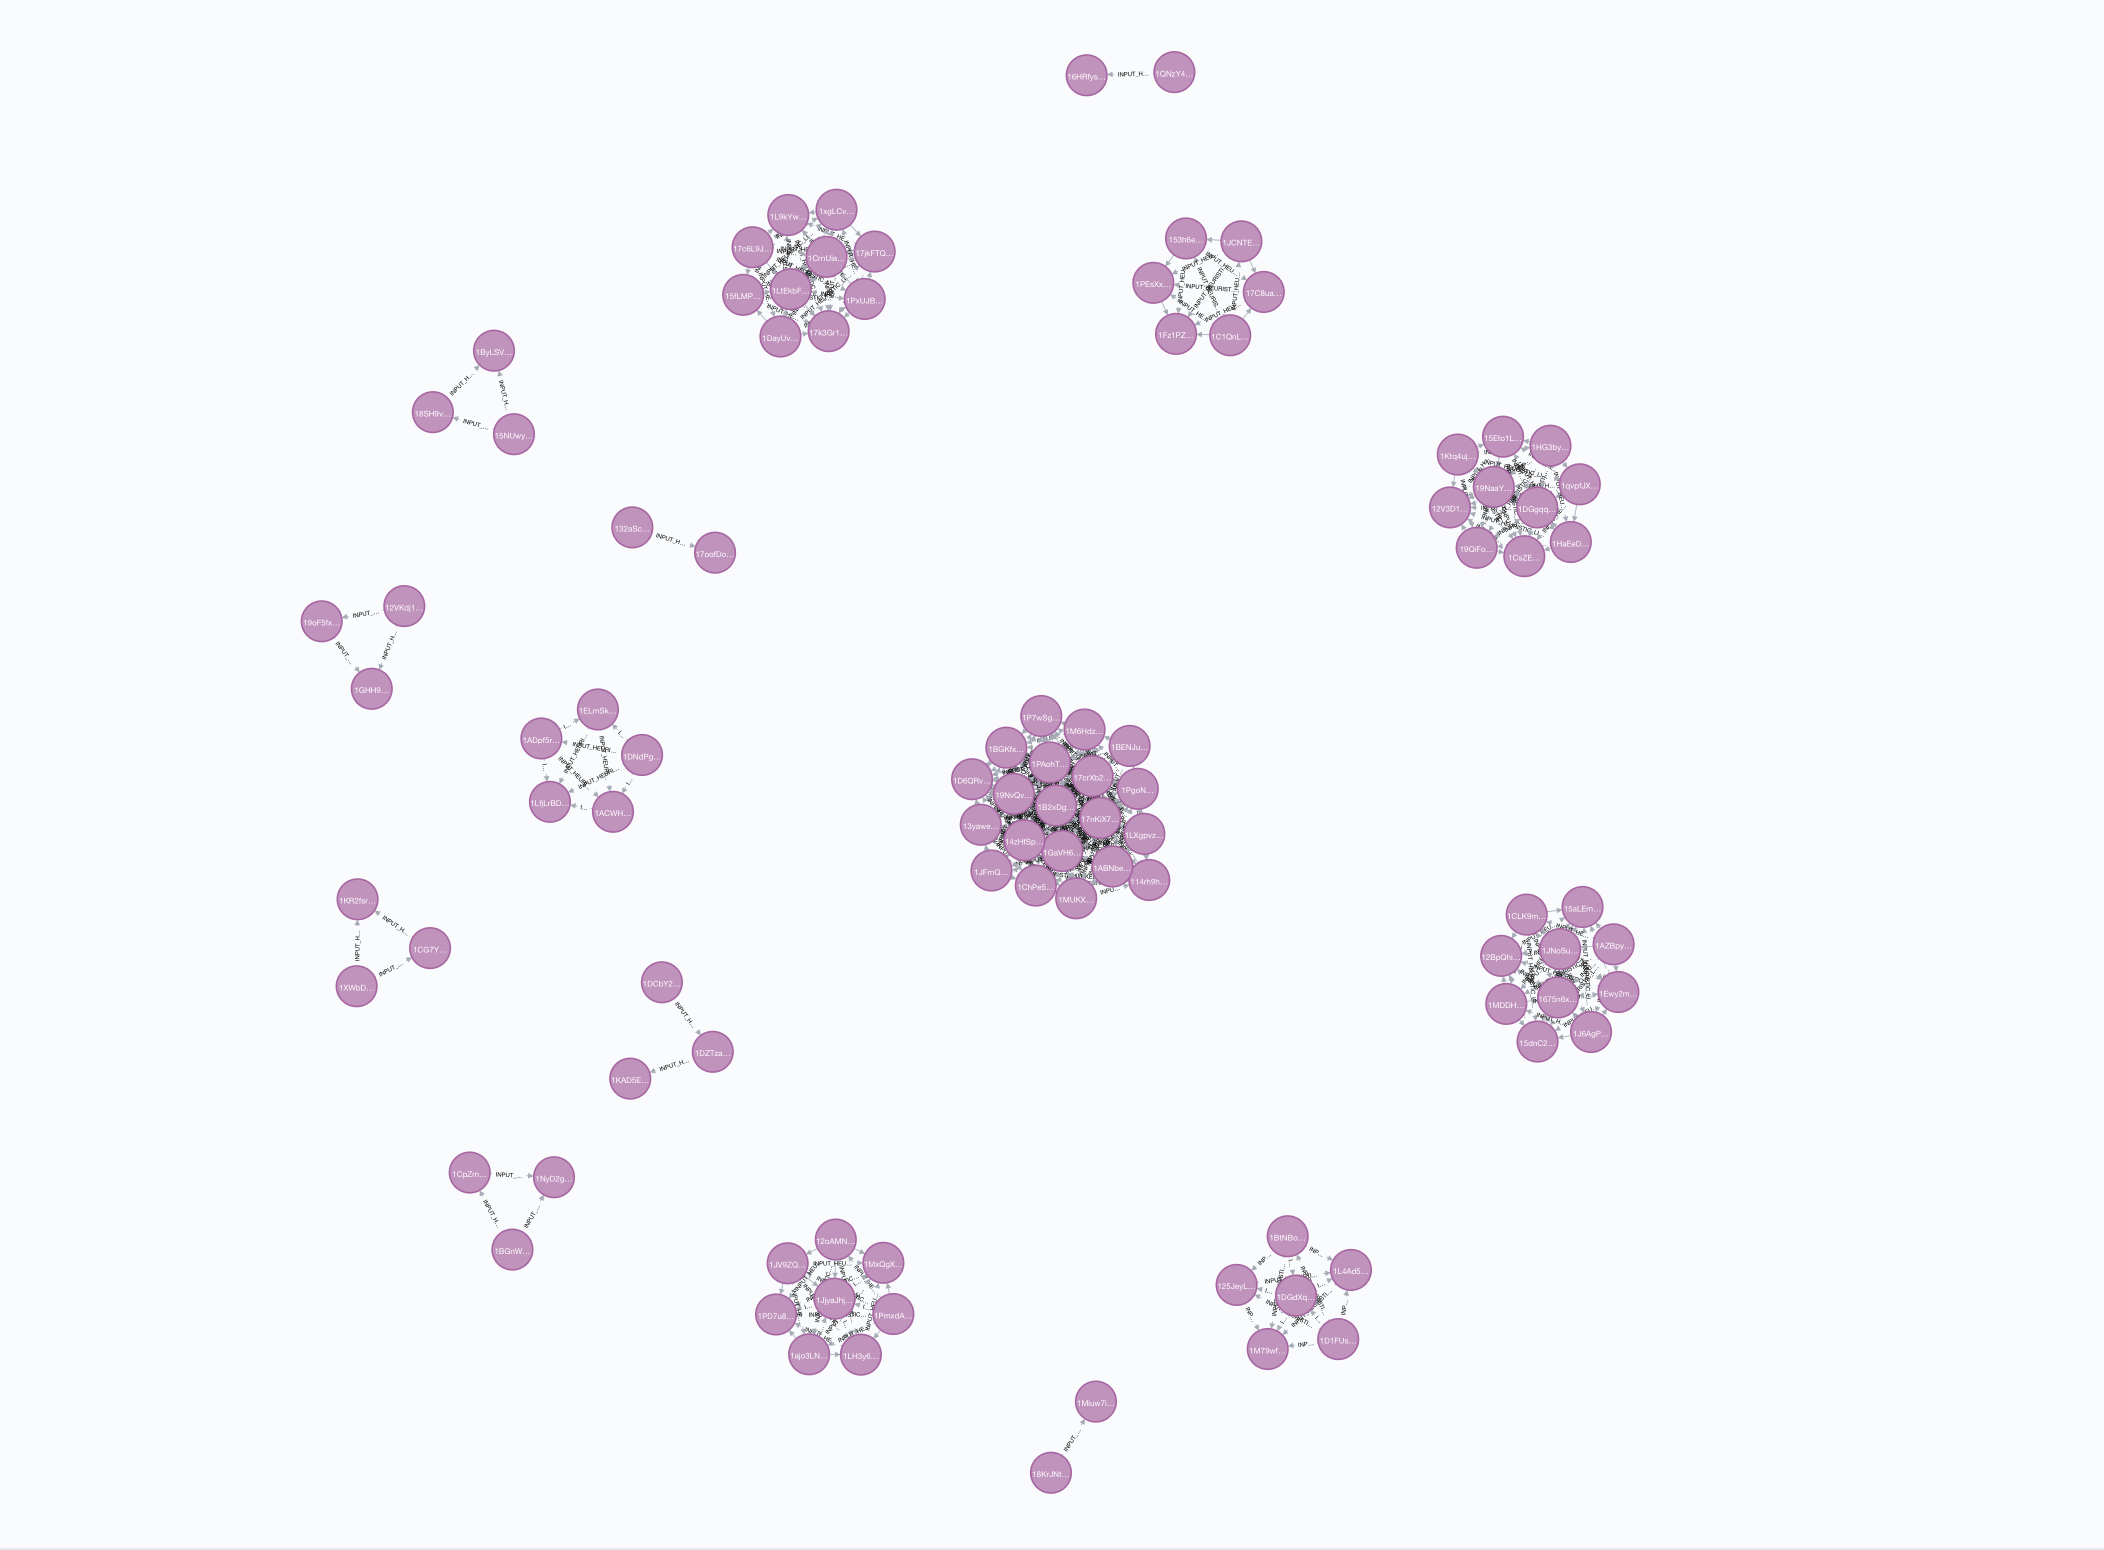
\includegraphics[width = 15cm]{./figures/many-clusters-heuristic-1}\\[0.5cm] 
  \caption{This shows my the Neo4J browser view of the several clusterings of addresses which all feed the same transaction.}
  \label{fig:neo4j-many-heuristic-1-clusters}
\end{figure}

\begin{figure}[h!]
  \centering
  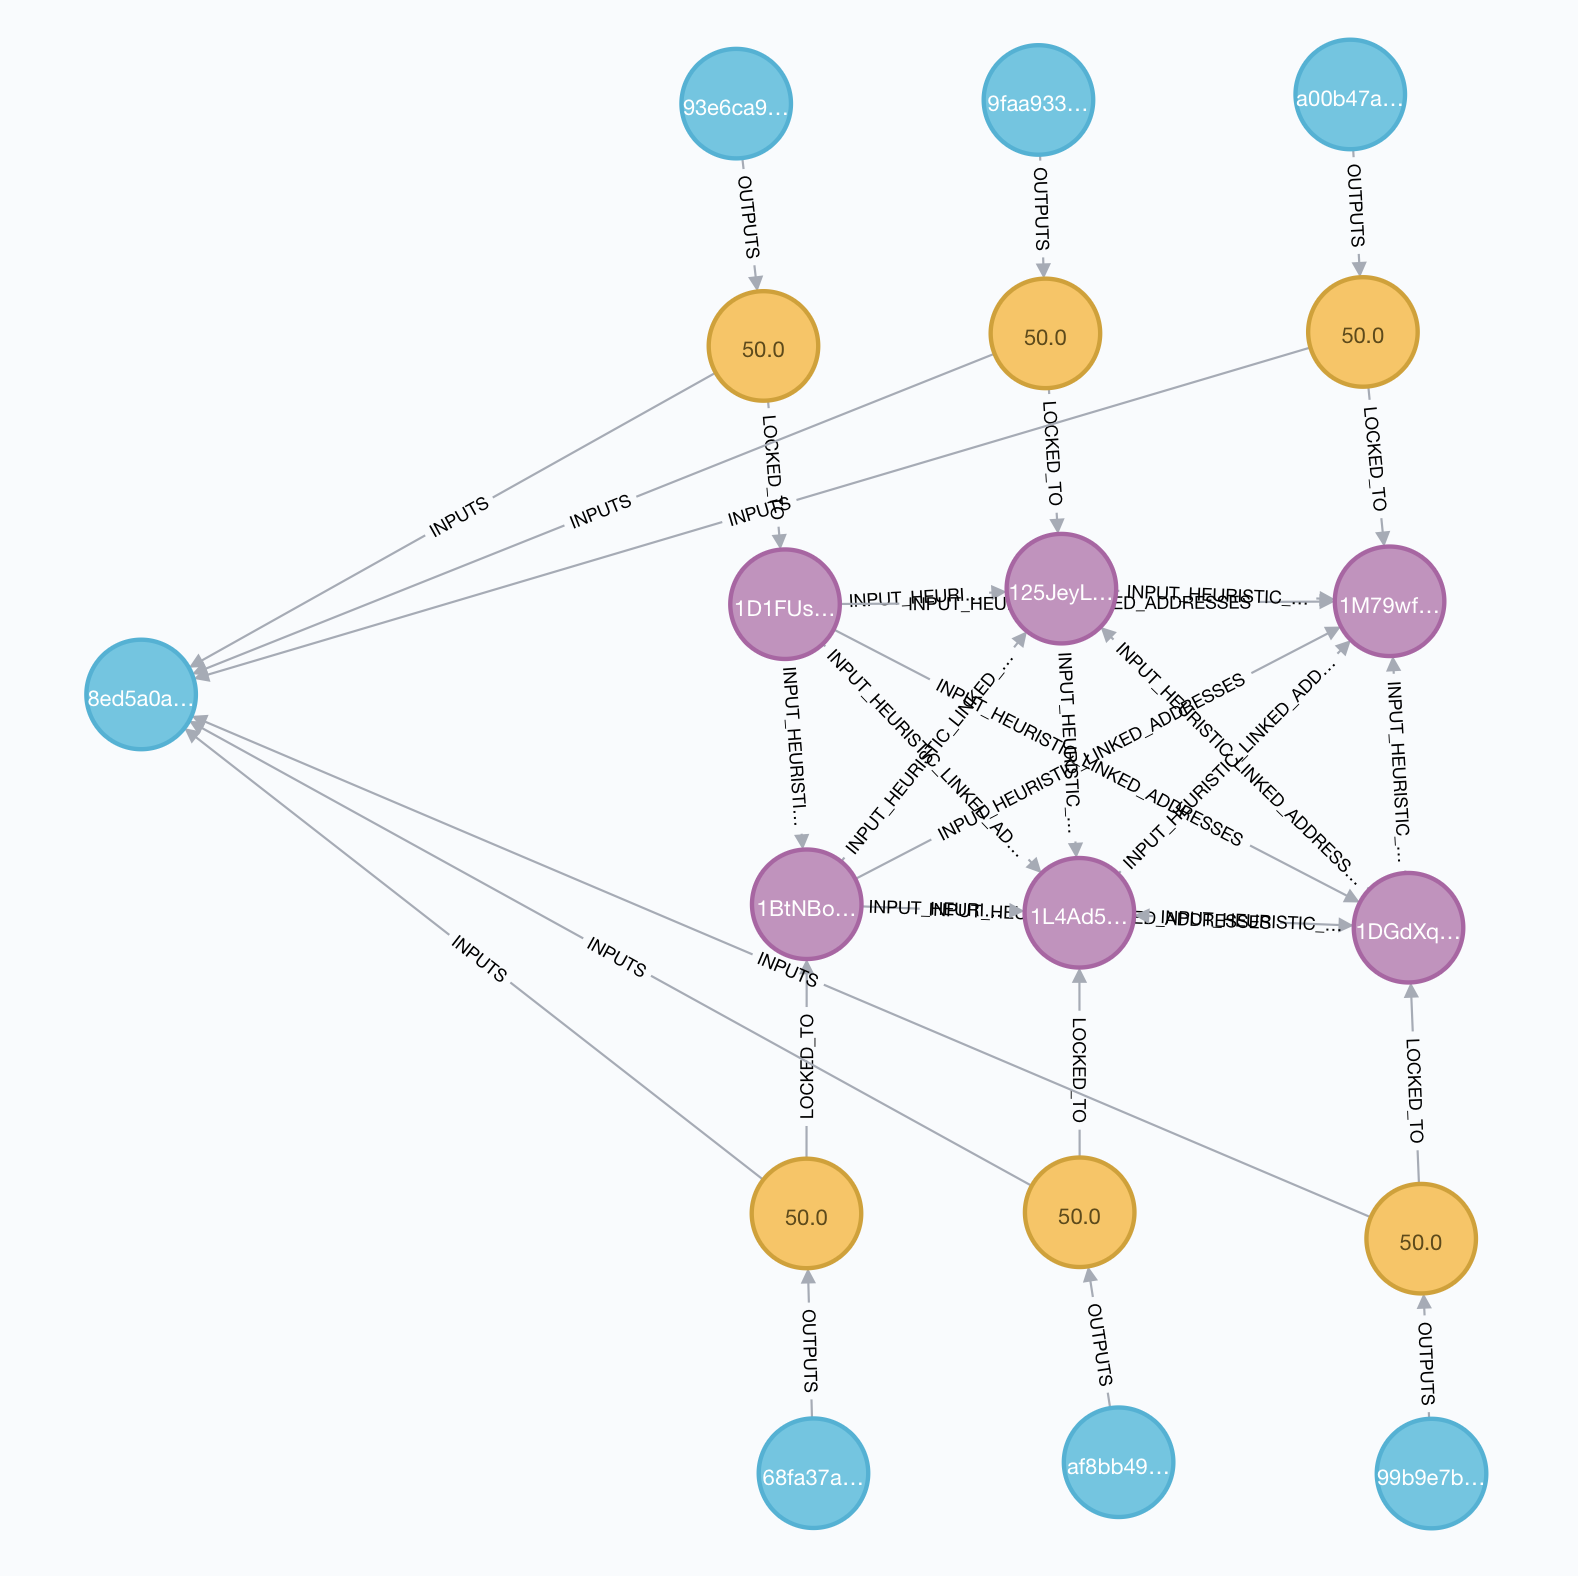
\includegraphics[width = 15cm]{./figures/input-one-tx-heuristic-1}\\[0.5cm] 
  \caption{This shows my the Neo4J browser view one one of the clusterings of addresses with their neighbours expanded to show they all have outputs locked to them which feed the same transaction}
  \label{fig:neo4j-1-tx-heuristic-1-cluster}
\end{figure}


\subsubsection{Efficiency}
Has to be serialisable: race condition when updating an address. An address could be the input for several transactions. There is therefore potential for interleaving address fetching, updating and saving leading to an incorrect state for an addresses links.  \todo{incomplete}

\subsection{Designing the change address heuristic}
\textbf{The idea:} This heuristic is based on an idiom of use in Bitcoin. When bitcoins from an output are spent in a transaction, they must be spent all at once, with the only way of dividing them up being through the use of a change address, where the excess input from the transaction is sent to a new address under the control of the sender \todo{Cite fistful}.

\textbf{Assumptions:} A change address only has \textbf{one} input. \\\\
\textbf{Robustness:} 
For each transaction, if multiple outputs meet the pattern of a change address, no address is labelled as the change address. A change address is labelled iff exactly one output meets the pattern. 
\begin{itemize}
    \item Avoid self-change addresses, where the change address is specified as the input address. 
    \item The address does not appear in any other transaction.
    \item The transaction is not a coin generation transaction. 
    \item All other output addresses have appeared in previous transactions.
\end{itemize}


 
\subsection{Performance issues} 
Searches for an address node using the tool takes an unacceptably long time (10 minutes 45 to find an Address node by its address and find its immediate neighbours). 

\subsubsection{Creating indexes}
Index's are useful for finding the starting point of a graph traversal. My tool requires exactly this functionality when we search for an address as the starting point of an investigation, before expanding out neighbours to traverse the blockchain. The initial search for the address is where the latency currently exists, therefore the first index I created was on the \texttt{address} property of the \texttt{ADDRESS} node. I was able to create this index by simply executing the command \texttt{CREATE INDEX ON :ADDRESS(address)} and using the command \texttt{CALL db.indexes} to track the progress of its population. 

Once the index was created, the search for an address returned almost immediately. However, when trying to expand the relations of the address neighbours, I encountered the same performance issues. I therefore had to create index's for the node properties which are used to fetch nodes.  


\subsubsection{Allocating more resources}
Neo4J provide a useful memory recommendation tool to suggest memory configuration parameters based on the size of a Neo4J database. 



    
    
\end{itemize}